%%%%%%%%%%%%%%%%%%%%%%%%%%%%%%%%%%%%%%%%%
% Short Sectioned Assignment
% LaTeX Template
% Version 1.0 (5/5/12)
%
% This template has been downloaded from:
% http://www.LaTeXTemplates.com
%
% Original author:
% Frits Wenneker (http://www.howtotex.com)
%
% License:
% CC BY-NC-SA 3.0 (http://creativecommons.org/licenses/by-nc-sa/3.0/)
%
%%%%%%%%%%%%%%%%%%%%%%%%%%%%%%%%%%%%%%%%%

%----------------------------------------------------------------------------------------
%	PACKAGES AND OTHER DOCUMENT CONFIGURATIONS
%----------------------------------------------------------------------------------------

\documentclass[paper=a4, fontsize=11pt]{scrartcl} % A4 paper and 11pt font size

\usepackage[T1]{fontenc} % Use 8-bit encoding that has 256 glyphs
\usepackage{fourier} % Use the Adobe Utopia font for the document - comment this line to return to the LaTeX default
\usepackage[english]{babel} % English language/hyphenation
\usepackage{amsmath,amsfonts,amsthm} % Math packages
\usepackage{listings}
\usepackage{graphicx}
%\graphicspath{ {Desktop/PA3_numerical_analysis/} }

\usepackage{lipsum} % Used for inserting dummy 'Lorem ipsum' text into the template

\usepackage{sectsty} % Allows customizing section commands
\allsectionsfont{\centering \normalfont\scshape} % Make all sections centered, the default font and small caps

\usepackage{fancyhdr} % Custom headers and footers
\pagestyle{fancyplain} % Makes all pages in the document conform to the custom headers and footers
\fancyhead{} % No page header - if you want one, create it in the same way as the footers below
\fancyfoot[L]{} % Empty left footer
\fancyfoot[C]{} % Empty center footer
\fancyfoot[R]{\thepage} % Page numbering for right footer
\renewcommand{\headrulewidth}{0pt} % Remove header underlines
\renewcommand{\footrulewidth}{0pt} % Remove footer underlines
\setlength{\headheight}{13.6pt} % Customize the height of the header

\numberwithin{equation}{section} % Number equations within sections (i.e. 1.1, 1.2, 2.1, 2.2 instead of 1, 2, 3, 4)
\numberwithin{figure}{section} % Number figures within sections (i.e. 1.1, 1.2, 2.1, 2.2 instead of 1, 2, 3, 4)
\numberwithin{table}{section} % Number tables within sections (i.e. 1.1, 1.2, 2.1, 2.2 instead of 1, 2, 3, 4)

\setlength\parindent{0pt} % Removes all indentation from paragraphs - comment this line for an assignment with lots of text

%----------------------------------------------------------------------------------------
%	TITLE SECTION
%----------------------------------------------------------------------------------------

\newcommand{\horrule}[1]{\rule{\linewidth}{#1}} % Create horizontal rule command with 1 argument of height

\title{	
\normalfont \normalsize 
\textsc{The College of William and Mary} \\ [25pt] % Your university, school and/or department name(s)
\horrule{0.5pt} \\[0.4cm] % Thin top horizontal rule
\huge Programming Assignment \#3 \\ % The assignment title
\horrule{2pt} \\[0.5cm] % Thick bottom horizontal rule
}

\author{Alexander Powell} % Your name

\date{\normalsize November 10, 2014} % Today's date or a custom date

\begin{document}
\lstset{language=MATLAB}

\maketitle % Print the title

%----------------------------------------------------------------------------------------
%	PROBLEM 1
%----------------------------------------------------------------------------------------

\section{}

The natural cubic spline of the parametric curve was found using the following MATLAB commands.  The functions {\textit{ncspline.m}} and {\textit{splineeval.m}} were used.  

\begin{lstlisting} [frame=single]
>> t = [0,1,2,3,4,5];
>> x = [1,1.5,2,2,2.5,2.5];
>> y = [1,0.5,1,1.5,1.5,1];
>> temp = 0:0.01:5;
>> [b1,c1,d1] = ncspline(t,x);
>> xx = splineeval(t,x,b1,c1,d1,temp);
>> [b2,c2,d2] = ncspline(t,y);
>> yy = splineeval(t,y,b2,c2,d2,temp);
>> figure
>> plot(xx,yy,x,y,'o'), axis equal, grid on
>> axis([.9,2.7,.4,1.65])
\end{lstlisting}

The following are tables of the natural cubic spline coeffients $a$, $b$, $c$, and $d$ for $t,x(t)$ and $t,y(t)$.  .  

\center{$a_j, b_j, c_j$ and $d_j$ values for $x(t)$}
%\begin{table} [H]
%\caption{Hello}
\begin{center}
  \begin{tabular}{ c || c | c | c | c }
    %\hline
    i & $a_i$ & $b_i$ & $c_i$ & $d_i$\\ \hline
    0 & 1   & 0.45215311 & 0          & 0.04784689 \\ \hline
    1 & 1.5 & 0.59569378 & 0.14354067 &-0.23923445 \\ \hline
    2 & 2   & 0.16507177 &-0.57416268 & 0.40909090 \\ \hline
    3 & 2   & 0.24401914 & 0.65311005 &-0.39712918 \\ \hline
    4 & 2.5 & 0.35885167 &-0.53827751 & 0.17942583 \\
    \hline
  \end{tabular}
\end{center}
%\end{table}


\center{$a_j, b_j, c_j$ and $d_j$ values for $y(t)$}
%\begin{table} [H]
%\caption{other}
\begin{center}
  \begin{tabular}{ c || c | c | c | c }
    %\hline
    i & $a_i$ & $b_i$ & $c_i$ & $d_i$\\ \hline
    0 & 1   &-0.76076555 & 0          & 0.26076555 \\ \hline
    1 & 0.5 & 0.02153110 & 0.78229665 &-0.30382775 \\ \hline
    2 & 1   & 0.67464114 &-0.12918660 &-0.04545454 \\ \hline
    3 & 1.5 & 0.27990430 &-0.26555023 &-0.01435406 \\ \hline
    4 & 1.5 &-0.29425837 &-0.30861244 & 0.10287081 \\
    \hline
  \end{tabular}
\end{center}
%\end{table}


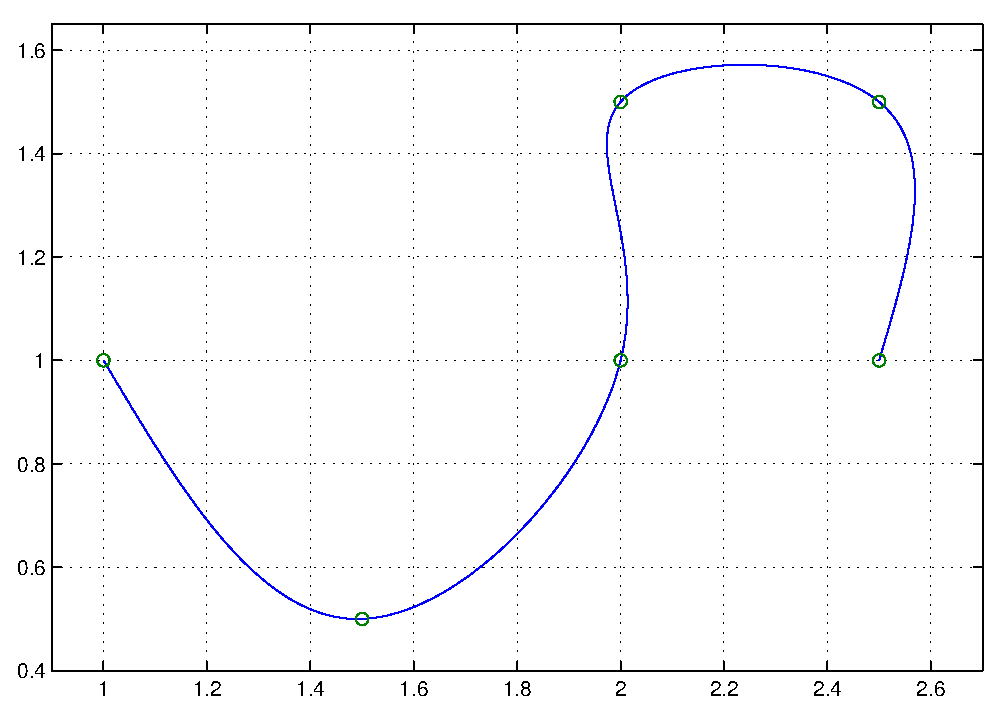
\includegraphics [scale=0.8] {myfig.eps}


%----------------------------------------------------------------------------------------
%	PROBLEM 2
%----------------------------------------------------------------------------------------

\bigskip
\bigskip
\bigskip
\bigskip
\bigskip
\bigskip
\bigskip
\bigskip
\bigskip
\bigskip
\bigskip
\bigskip
\bigskip

\section{}

Newton's method was used to estimate the parameter values $t_1$ and $t_2$ where the curve intersects the line $y = 1.2$.  The following MATLAB code was used to make the calculations:

\begin{lstlisting} [frame=single]
t = [0,1,2,3,4,5];
x = [1,1.5,2,2,2.5,2.5];
y = [1,0.5,1,1.5,1.5,1];
temp = 0:0.01:5;
[b1,c1,d1] = ncspline(t,x);
[b2,c2,d2] = ncspline(t,y);
CountMax = 100;
guess = 2; % 2 was the guess for the left, 5 for the right
x_p = guess;
tol = 1e-8;
for i=1:CountMax
	guess = guess - (splineeval(t,y,b2,c2,d2,guess)-1.2) / 
    diffsplineeval(t,y,b2,c2,d2,guess); 
    % the above two lines are actually one line but 
    % are separated for readability.  
	
	if (splineeval(t,y,b2,c2,d2,guess) < tol & abs(guess-x_p) < tol)
	    fprintf( 'x%d = %.15f\n', i, guess );
	    disp(['It took ' num2str(i) ' steps to converge.' ])
	    return;
	else
	    fprintf( 'x%d = %.15f\n', i, guess );
	    x_p = guess;
	end
end
disp('Reach the maximum number of iterations!');
\end{lstlisting}

The above code generated the following values:
$$t_1 = 2.31798217, t_2 = 4.66164416$$

%----------------------------------------------------------------------------------------

% ----------Problem 3 -------------------------

\bigskip
\bigskip
\bigskip
\bigskip
\bigskip
\bigskip
\bigskip
\bigskip
\bigskip
\bigskip

\section{}


The following code computes the length of the curve by using the composite trapezoid rule with increasingly greater values of $n$.  

\begin{lstlisting} [frame=single]
ns = [16, 32, 64, 128, 10000];
t = [0,1,2,3,4,5];
x1 = [1,1.5,2,2,2.5,2.5];
y1 = [1,0.5,1,1.5,1.5,1];
[b1,c1,d1] = ncspline(t,x1);
[b2,c2,d2] = ncspline(t,y1);

f = @(x) sqrt(((diffsplineeval(t,x1,b1,c1,d1,x)).^2
+ ((diffsplineeval(t,y1,b2,c2,d2,x)).^2));
% ^these are one line in MATLAB but were separated for clarity

a = 2.31798217; b = 4.66164416;
for n = ns
    x = linspace(a, b, n+1);
    h = (b-a)/n;
    int = (h/2)*(2*sum(f(x)) -f(a) - f(b))
end
\end{lstlisting}


\begin{flushleft}
The following is a table displaying the different approximations:
\end{flushleft}

\begin{center}
  \begin{tabular}{ | c | c | }
    \hline
    $L_{16}    $ & 1.16265486  \\ \hline
    $L_{32}    $ & 1.16178581  \\ \hline
    $L_{64}    $ & 1.16160475  \\ \hline
    $L_{128}   $ & 1.16155626  \\ \hline
    $L_{10000} $ & 1.16154051  \\
    \hline
  \end{tabular}
\end{center}

The following is a log-log plot of the errors $\mid L_n - L \mid$ versus $h = (t_1 - t_2) / n$.  

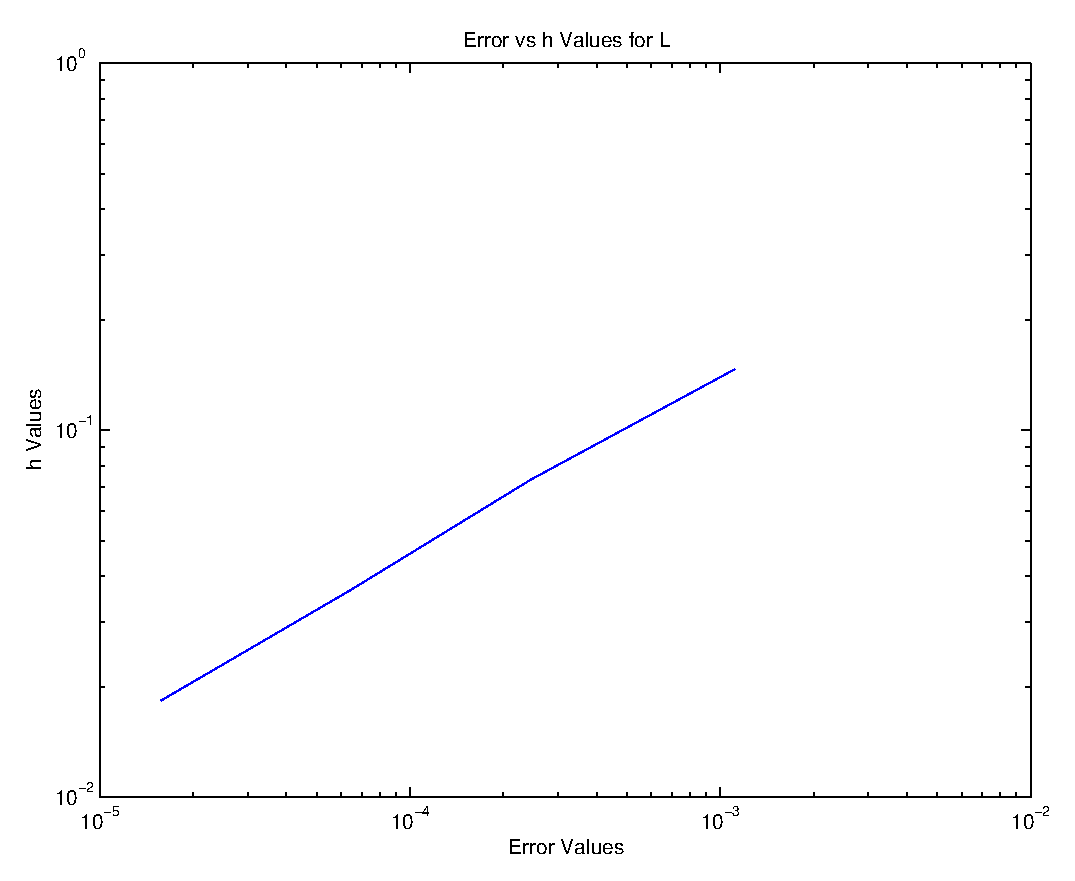
\includegraphics [scale=0.8] {prob2fig.eps}

\begin{flushleft}
Applying the log-log plot changes the figure almost to a line.  Using the ordered pairs $(10^{-3}, 10^{-0.9})$ and $(10^{-4},10^{-1.5})$ gives us:
\end{flushleft}
$$\frac{10^{-1.5}-10^{-0.9}}{10^{-4}-10^{-3}} \approx 100$$

\begin{flushleft}
So, the slope of the log-log plot is approximately $100$.  
\end{flushleft}





% -----------end document --------------------
\end{document}